\documentclass[journal,onecolumn]{IEEEtran}
\usepackage{header}

\usepackage[portuguese]{babel}
% \usepackage[backend=biber]{biblatex}
% \addbibresource{references.bib}

\title{
    TP4: Análise Quantitativa do Trade-off entre Especialização e Generalização em LLMs via Fine-Tuning
}

\author[1]{Lucas Castro de Souza \thanks{lucas.castro@icomp.ufam.edu.br}}
\affil[1]{Universidade Federal do Amazonas - PPGI}

\newcommand{\figwidth}{0.7\linewidth}

\begin{document}

\maketitle
\IEEEpeerreviewmaketitle

%1. Objetivo
% O objetivo central deste projeto é a avaliação empírica e sistemática do processo de fine-tuning em Modelos de Linguagem de Grande Porte (LLMs).
% Os alunos irão implementar, treinar e avaliar um LLM para a tarefa de Text-to-SQL. A análise quantificará o ganho de desempenho na tarefa-alvo e,
% simultaneamente, medirá a degradação de performance em tarefas de conhecimento geral. O projeto exige a implementação de métricas de
% avaliação customizadas e uma análise crítica dos trade-offs inerentes à especialização de modelos.
% 2. Problema
% A especialização de LLMs via fine-tuning é uma técnica proposta para otimizar o desempenho em domínios específicos. Contudo, este
% processo de otimização focado pode comprometer a robustez do modelo em tarefas que não pertencem ao domínio de treinamento, um
% fenômeno conhecido como "esquecimento catastrófico" ou "regressão de capacidade". Esse trabalho consiste em projetar e executar
% um pipeline experimental que permita medir com precisão ambas as facetas deste fenômeno: o ganho de especialização e a perda de
% generalização.
% 3. Materiais e Configuração
% ● Modelo Base: Deve ser utilizado um modelo open-source da classe de 7-8 bilhões de parâmetros em sua versão instruct/chat. Modelos
% sugeridos: meta-llama/Llama-3-8B-Instruct, mistralai/Mistral-7B-Instruct-v0.2. A versão exata do checkpoint utilizado
% deve ser documentada para garantir a reprodutibilidade.
% ● Dataset de Fine-Tuning: Spider Dataset, disponível no site oficial. Utilizar exclusivamente o training split. Os dados devem ser
% pré-processados para o formato exigido pelo framework de treinamento escolhido (e.g., formato de chat com [INST], [SYS]).
% ● Dataset de Avaliação de Tarefa: Spider development split. Este conjunto de dados não deve ser visto pelo modelo durante o treinamento.
% ● Dataset de Avaliação de Generalização: MMLU (Massive Multitask Language Understanding), disponível no Hugging Face Hub. Deve ser
% criada uma suíte de avaliação composta por exatamente 150 questões, divididas igualmente em 3 categorias:
% 1. STEM: 50 questões de uma subcategoria (e.g., computer_science).
% 2. Humanidades: 50 questões de uma subcategoria (e.g., philosophy).
% 3. Ciências Sociais: 50 questões de uma subcategoria (e.g., economics).
% ● Framework de Avaliação: DeepEval (versão 0.21.x ou superior).
% ● Frameworks de Treinamento: Hugging Face TRL, Axolotl ou similar

\section{Introdução}
Este trabalho propõe uma análise quantitativa do impacto do fine-tuning supervisionado em LLMs, utilizando a tarefa de Text-to-SQL como estudo de caso. O objetivo é mensurar, de forma sistemática, tanto o ganho de desempenho na tarefa-alvo quanto a degradação da capacidade de generalização em benchmarks de conhecimento geral, evidenciando o trade-off inerente ao processo de especialização de grandes modelos de linguagem.

\section{Metodologia}
 A seguir, está detalhada cada etapa do pipeline experimental deste trabalho, incluindo arquitetura dos scripts, o pré-processamento dos dados, configuração do modelo base, a configuração do treinamento com LoRA, e a implementação da métrica customizada de avaliação.

\subsection{Arquitetura dos Scripts}

O projeto foi organizado em seis scripts principais. Cada um é responsável por uma etapa específica do pipeline experimental, eles foram executados na mesma ordem em que são apresentados aqui. A seguir, uma breve descrição de cada script:

\begin{itemize}
    \item \textbf{0\_preparando\_dados.py}: Responsável pelo pré-processamento dos dados. Este script carrega o Spider dataset, extrai e formata os exemplos para o formato de chat utilizado no fine-tuning e avaliação. Também prepara e salva o conjunto de questões do MMLU, garantindo a divisão correta por categorias.

    \item \textbf{1\_fine-tuning.py}: Realiza o treinamento supervisionado do modelo base utilizando LoRA. Implementa o pipeline de tokenização, configuração dos hiperparâmetros do LoRA, argumentos de treinamento e execução do processo de fine-tuning, salvando checkpoints intermediários.

    \item \textbf{2\_calculando\_baseline.py}: Calcula o desempenho de baseline do modelo base (sem fine-tuning) na tarefa de Text-to-SQL. Utiliza exemplos 3-shot e executa as queries geradas, comparando com as respostas de referência para medir a acurácia inicial.

    \item \textbf{3\_avaliacao\_customizada.py}: Avalia os modelos fine-tuned utilizando a métrica customizada \textit{ExecutionAccuracy} utilizando o framework DeepEval. Gera prompts, executa as queries SQL produzidas pelo modelo e compara os resultados com o ground truth, salvando checkpoints e resultados detalhados.

    \item \textbf{4\_analise\_mmlu.py}: Mede a generalização dos modelos (base e fine-tuned) no benchmark MMLU. Gera prompts 4-shot para questões de múltipla escolha, executa a inferência e calcula métricas de acurácia e desvio padrão por categoria.
\end{itemize}

Para garantir a reprodutibilidade dos experimentos, todos os seeds dos geradores de números aleatórios foram fixados em 42. Sempre que possível, opções determinísticas foram selecionadas nos frameworks utilizados para minimizar variações entre execuções.

\subsection{Pré-processamento dos Dados}
O pré-processamento dos dados é necessário para garantir a compatibilidade dos datasets com o modelo e os frameworks utilizados. Inicialmente, o Spider dataset foi carregado a partir do arquivo original \texttt{dev.json}. Para cada entrada, foi extraída a questão em linguagem natural, a query SQL de referência e o esquema do banco de dados correspondente. O esquema foi reconstruído em formato textual, listando todas as tabelas e colunas presentes no banco, de modo a fornecer ao modelo o contexto necessário para a geração da query. Veja a Figura~\ref{fig:spider_processed} para um exemplo de entrada do Spider dataset após o pré-processamento.

\begin{figure}[!htpb]
    \centering
    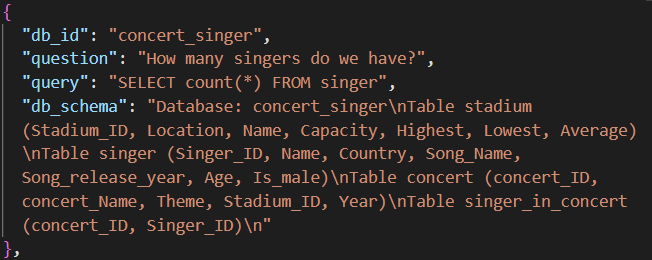
\includegraphics[width=\figwidth]{resources/spider_processed.png}
    \caption{Exemplo de entrada do Spider dataset após pré-processamento}
    \label{fig:spider_processed}
\end{figure}

Cada exemplo foi então convertido para o formato de chat, seguindo o padrão de prompts utilizado por modelos da família Qwen. O prompt inclui um bloco \texttt{system} com a instrução geral, um bloco \texttt{user} contendo o esquema do banco e a questão, e um bloco \texttt{assistant} com a query SQL de referência (no caso do treinamento) ou vazio (no caso da inferência). A Figura~\ref{fig:spider_prompt} ilustra a função que cria o prompt de inferência para uma consulta do Spider.

\begin{figure}[!htpb]
    \centering
    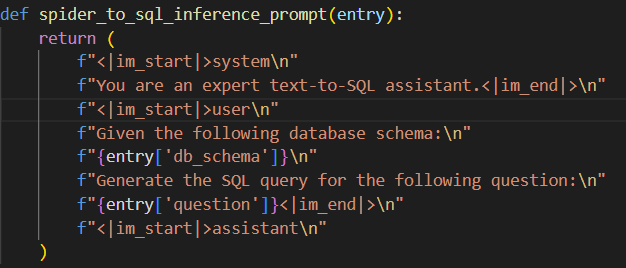
\includegraphics[width=\figwidth]{resources/spider_prompt.png}
    \caption{Função que cria um prompt de inferência para uma consulta do Spider.}
    \label{fig:spider_prompt}
\end{figure}

Para a avaliação de generalização, foi utilizada uma amostra de 150 questões do benchmark MMLU, divididas igualmente entre as categorias STEM (elementary\_mathematics), Humanidades (philosophy) e Ciências Sociais (management). As questões foram selecionadas de subcategorias específicas e processadas para o formato de prompt compatível, incluindo o enunciado da questão e as alternativas de resposta. A Figura~\ref{fig:mmlu_processed} ilustra o formato de uma questão do MMLU após o processamento.
\begin{figure}[!htpb]
    \centering
    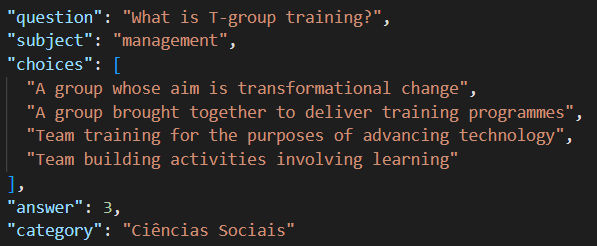
\includegraphics[width=\figwidth]{resources/mmlu_processed.png}
    \caption{Formato de uma questão do MMLU após ser processada.}
    \label{fig:mmlu_processed}
\end{figure}

\subsection{Configuração do Modelo Base}

O modelo base utilizado neste experimento foi o \texttt{Qwen/Qwen2-7B-Instruct}. A escolha deste modelo se deve a ser um modelo de 7 bilhões de parametros e ter boa performance no benchmark MMLU-Pro.

Ele foi carregado de forma quantizada pois ele não cabe sem quantização na GPU grátis do Google Colab (T4 15GB), que foi utilizada para o treinamento e avaliação. Foi utilizado também, \texttt{float16} pois a GPU grátis do Google Colab não suporta \texttt{bfloat16}. Veja Figura~\ref{fig:base_model_config} para detalhes da configuração de carregamento do modelo.

\begin{figure}[!htpb]
    \centering
    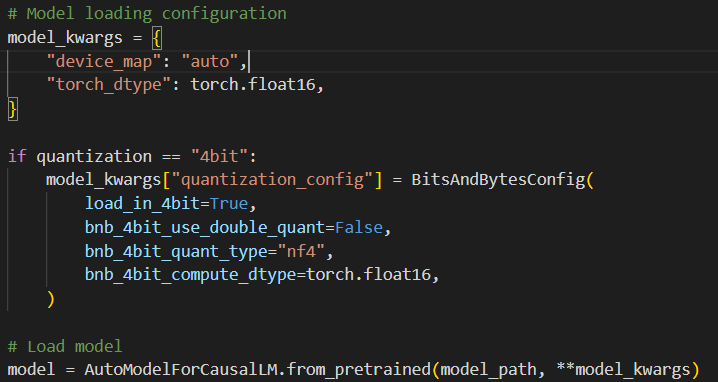
\includegraphics[width=\figwidth]{resources/base_model_config.png}
    \caption{Configuração de carregamento do modelo em modo quantizado.}
    \label{fig:base_model_config}
\end{figure}


\subsection{Configuração do Treinamento com QLoRA}

O fine-tuning foi realizado utilizando o método QLoRA (Quantized Low-Rank Adaptation). Foram adaptados apenas os módulos de atenção do modelo (\texttt{q\_proj}, \texttt{k\_proj}, \texttt{v\_proj}, \texttt{o\_proj}), reduzindo o número de parâmetros treináveis e acelerando o processo de fine-tuning. A configuração do LoRA adotada está detalhada na Figura~\ref{fig:lora_config}.

\begin{figure}[!htpb]
    \centering
    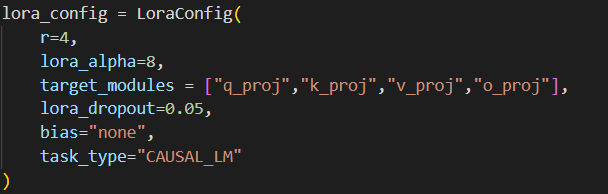
\includegraphics[width=\figwidth]{resources/lora_config.png}
    \caption{Configuração LoRA.}
    \label{fig:lora_config}
\end{figure}

\subsection{Configuração do Treinamento}

O treinamento foi conduzido por 5 épocas, com batch size efetivo de 8 (batch size 2 e \textit{gradient accumulation steps} 4), taxa de aprendizado inicial de $2 \times 10^{-4}$, otimizador AdamW em modo 8-bit.

Os checkpoints do LoRA foram salvos a cada época para permitir a avaliação do finetuning em diferentes épocas, como pedido na especificação do trabalho. Veja a Figura~\ref{fig:training_config} para detalhes da configuração do treinamento.

\begin{figure}[!htpb]
    \centering
    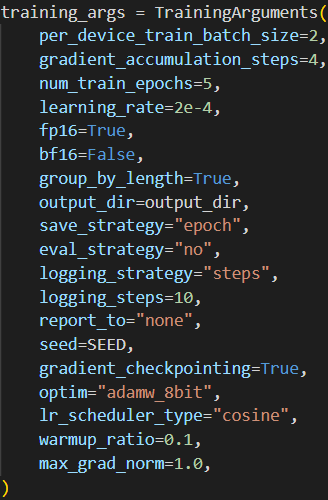
\includegraphics[width=0.25\linewidth]{resources/training_config.png}
    \caption{Configuração do Treinamento.}
    \label{fig:training_config}
\end{figure}

\subsection{Implementação da Métrica Customizada: ExecutionAccuracy}

Para avaliar a geração de consultas SQL, foi implementada a métrica customizada \textbf{ExecutionAccuracy}, compatível com o framework DeepEval. Essa métrica executa tanto a query gerada pelo modelo quanto a de referência no mesmo banco SQLite, atribuindo score 1.0 se os resultados coincidirem (ignorando ordem e duplicatas) e 0.0 caso contrário ou em caso de erro de execução. Mensagens de erro são registradas para análise posterior. A Figura~\ref{fig:custom_metric_main} mostra o núcleo da implementação.
\begin{figure}[!htpb]
    \centering
    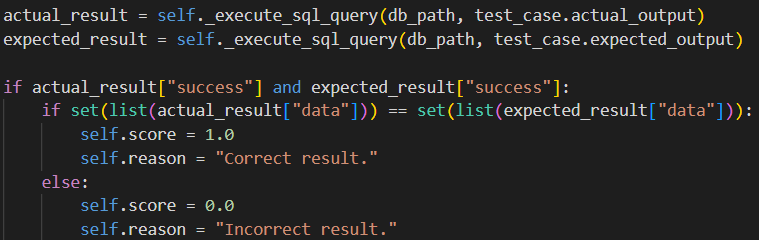
\includegraphics[width=\figwidth]{resources/custom_metric_main.png}
    \caption{Parte principal da função que avalia os resultados.}
    \label{fig:custom_metric_main}
\end{figure}

% add new figure
\section{Resultados}
% Os resultados devem ser apresentados com clareza estatística (e.g., médias, desvio padrão). É fortemente recomendada a inclusão de uma breve análise de erros, examinando 2-3 exemplos onde o modelo fine-tuned falhou na tarefa-alvo.

\section{Discussão}
% A análise deve ser aprofundada, respondendo a perguntas como: A magnitude do ganho na tarefa de Text-to-SQL justifica a perda de capacidade geral? Quais fatores (hiperparâmetros, arquitetura do modelo) parecem influenciar mais este trade-off? Quais são as implicações práticas destes achados para o desenvolvimento de LLMs comerciais especializados?


% \printbibliography

\end{document}
